\section{Manipulation Methods}
\label{sec:manipulation_methods}

As outlined in \autoref{sec:interpretation_methods}, there are a variety of explanation methods readily available as frameworks and open source implementations. However, there is still little analysis on the robustness and reliability of such methods. 
While it is already common practice to test machine learning models against adversarial attacks in a number of domains \cite{gao2019universal, kereliuk2015deep}, the same is not yet the standard for interpretation methods. We argue that interpretation techniques should not be used in critical applications without basic testing of interpretation techniques against adversarial settings.

\subsection{Adversarial Setting}
\label{subsec:adversarial_setting}
\mypar{Adversarial Attacks on Models. }
Adversarial examples, as first introduced by \cite{szegedy_intriguing}, are clever manipulations of an input by an adversary which aims at causing misclassification and fooling of applications. They are mostly used to fool or attack machine learning models. We formally define adversarial attacks by the following properties: 
\par\smallskip
\textbf{Definition 2: Model Manipulation Method}
\begin{enumerate}
    \item[1.] \textit{Imperceptibility of Perturbation}: The adversarial example is similar to original data, i.e. the norm of the added perturbation $\delta$ to an input sample $\mathbf{x}$ thus must be small, i.e. $$\norm{\mathbf{x}+\delta} = \norm{(\mathbf{x}+\delta)-\mathbf{x}}_{\inf} \leq \epsilon$$
    \item[2.] \textit{Prediction dissimilarity}: The prediction of the model is significantly different to the prediction on the non-adversarial example: $$f_N(\mathbf{x}+\delta) \approx f_N(\mathbf{x})$$
\end{enumerate}
Note, that within adversarial fooling of models, the perturbation is mostly applied to the input data, and not to the model itself.

% TODO cite
Evidence from many studios shows that deep learning models can be easily tricked by adversarial examples. 
Albeit there are not yet as many studies, there also exists evidence that many interpretation methods are also fragile with respect to small changes to input data \cite{adebayo2018sanity, samek2019explainable, alvarez2018towards} as well as to the model itself \cite{fooling_nn_interpreters, dimanov2020you}. This fooling of interpretation methods is outlined below. 

\mypar{Adversarial Attacks on Model Interpreters.} 
Contrary to adversarial attacks on machine learning models, the focus of this paper is on the attacks on interpretation techniques without changing the prediction of the model. 
An adversarial attack on a model interpretation is in the following also called a \textit{manipulation} method. 
The goal is to apply perturbations to either an input sample or the model to change the output of an interpretation technique while leaving the model prediction unchanged. The last condition is important because adversarial interpreter manipulations aim to fool the interpretation method and essentially not the model itself. 
Fooling the model would only disclose the vulnerability of the model but would not allow to gain insight into the stability \footnote{Stability is given if a method yields consistent outcomes in independent runs.} of the interpretation method.

Again, the problem can be formally defined as:

% A manipulation method refers to a method influencing an interpretation method $\mathcal{I}$ to yield a wrong interpretation. This influence on the interpretation method is also called \textit{fooling} or an \textit{attack}. 
\par\smallskip
\textbf{Definition 3: Interpretation Manipulation Method.}

\setlength{\leftskip}{0.39cm}
% as it is the goal to disclose the vulnerability of the explanation method and not the vulnerability of the model.
\noindent A manipulation method $\mathcal{F}$ is defined as a method for altering the output of an explanation method $\mathcal{I}$ while leaving the model performance of the neural network $N$ roughly unchanged. 
As manipulations can be applied on the input or the model level (see \autoref{subsubsec:manipulation_levels}), $\mathbf{x}+\delta$ denotes a perturbed input sample regarding the input level manipulation, while $N+\delta$ denotes a model with altered parameters, referring to the model level manipulation.

A manipulation method is successful in fooling an interpreter, if the following properties hold: 
\begin{enumerate}
    % TODO for all i, as in http://lcfi.ac.uk/media/uploads/files/DimanovBhattJamnikWeller_YouShouldntTrustMe.pdf 
    \item[1.] \textit{Prediction similarity}: The model prediction stays approximately the same, i.e. $$f_N(\mathbf{x}+\delta) \approx f_N(\mathbf{x}) \text{, or } f_{N+\delta}(\mathbf{x}) \approx f_N(\mathbf{x})$$
    % \item[2.] \textit{Interpretation dissimilarity}: The explanation map $h(\mathbf{x}+\delta)$ is significantly different to the explanation map resulting from non adversarial models or inputs $h(\mathbf{x})$, i.e. $h(\mathbf{x}+\delta)$ or $$\argmax_{\delta} = \mathcal{D}(\mathcal{I}(x_i, \boldsymbol{\omega}), \mathcal{I}(x_i+\delta, \boldsymbol{\omega})$$
    \item[2.] \textit{Imperceptibility of Perturbation}: In case the attack is in the input domain of the model, the perturbation of input samples must be imperceptible by humans. According to \cite{dombrowski2019explanations}, the norm of the added perturbation $\delta$ to an input sample $\mathbf{x}$ thus must be small, i.e. $$\norm{\mathbf{x}+\delta} = \norm{(\mathbf{x}+\delta)-\mathbf{x}}_{\inf} \leq \epsilon$$ % https://arxiv.org/pdf/1710.10547.pdf 
\end{enumerate}
\setlength{\leftskip}{0cm}

These measures are to be seen as comparison between a baseline model $N$ and a model that is applied an the adversarial setting (i.e. either $N$ is not changed but applied to adversarially altered data $x+\delta$, or $N$ is adversarially trained thus becoming $N+\delta$). 
Interpretation manipulation methods differ with respect to the definition of the fooling of the interpretation method. 
Some methods aim to make the interpreter give wrong interpretations\cite{fooling_nn_interpreters}. 
In this case, the following additional property must hold: 
\begin{enumerate}
   \item[3.] \textit{Interpretation dissimilarity}: The explanation map $h(\mathbf{x}+\delta)$ is significantly different to the explanation map resulting from non adversarial models or inputs $h(\mathbf{x})$, i.e. $h(\mathbf{x}+\delta)$ or $$\argmax_{\delta} \mathcal{D}(\mathcal{I}(x_i, \boldsymbol{\omega}), \mathcal{I}(x_i+\delta, \boldsymbol{\omega}))$$ where $\mathcal{D}(\cdot)$ is a distance measure. 
\end{enumerate}

Others introduce a systematic bias into tho model while fooling the interpretation method in the sense that the interpretation does not change between the original model and the adversarial model. 
Here, it must hold that property 3. takes the minimal argument.
% TODO add image for this. 

\cite{dimanov2020you} extend these properties to include the so called \textit{model similarity}. This measure extends the \textit{prediction accuracy} to span the accuracy difference in between the baseline model and the new model, and also the mismatch of data points where the predictions of both models differ. 

After formally defining what successfully fooling an interpretation method means, we want to provide intuition in \autoref{fig:lrp_cat}. The interpretation method produces an interpretation, here in form of a saliency map projected onto the original image. If a successful manipulation is applied, the resulting saliency map of the same interpreter should be different to the original map. This effect is clearly visible, as \autoref{fig:lrp_cat_lrp} is visually significantly different to the map produced by the same interpretation method but applied to an adversarial model (see \autoref{fig:lrp_cat_fooled_lrp}). 

%%%%%%%%%%%%%%%%%%%%%%%%%
\subsection{Taxonomy of Interpretation Manipulation Methods}
\label{subsec:taxonomy_manipulations}
There are two important categories of Manipulation Methods that aim at attacking model interpretation methods. The first category is based on the level these manipulations operate on, i.e. input space level or model / parameter level. 
The second categorization is based on the target of the manipulations. While untargeted manipulations are mostly random perturbations, targeted manipulations aim to perturb the interpretation of specific input features. 

%%%%%%%%%%
\subsubsection{Manipulation Levels}
\label{subsubsec:manipulation_levels}
\par\smallskip
\noindent 

\par\smallskip
\noindent\textbf{Adversarial Input Manipulation.} The general approach is to perturb or alter input data while observing the effect of this perturbation on the model prediction. This concept is visualized in \autoref{fig:input_manipulation}. 
As found in \cite{dombrowski2019explanations}, visually-imperceptible perturbations of an input image can make explanations worse for the same model and interpreter. 

\begin{figure}[ht]
    \centering
    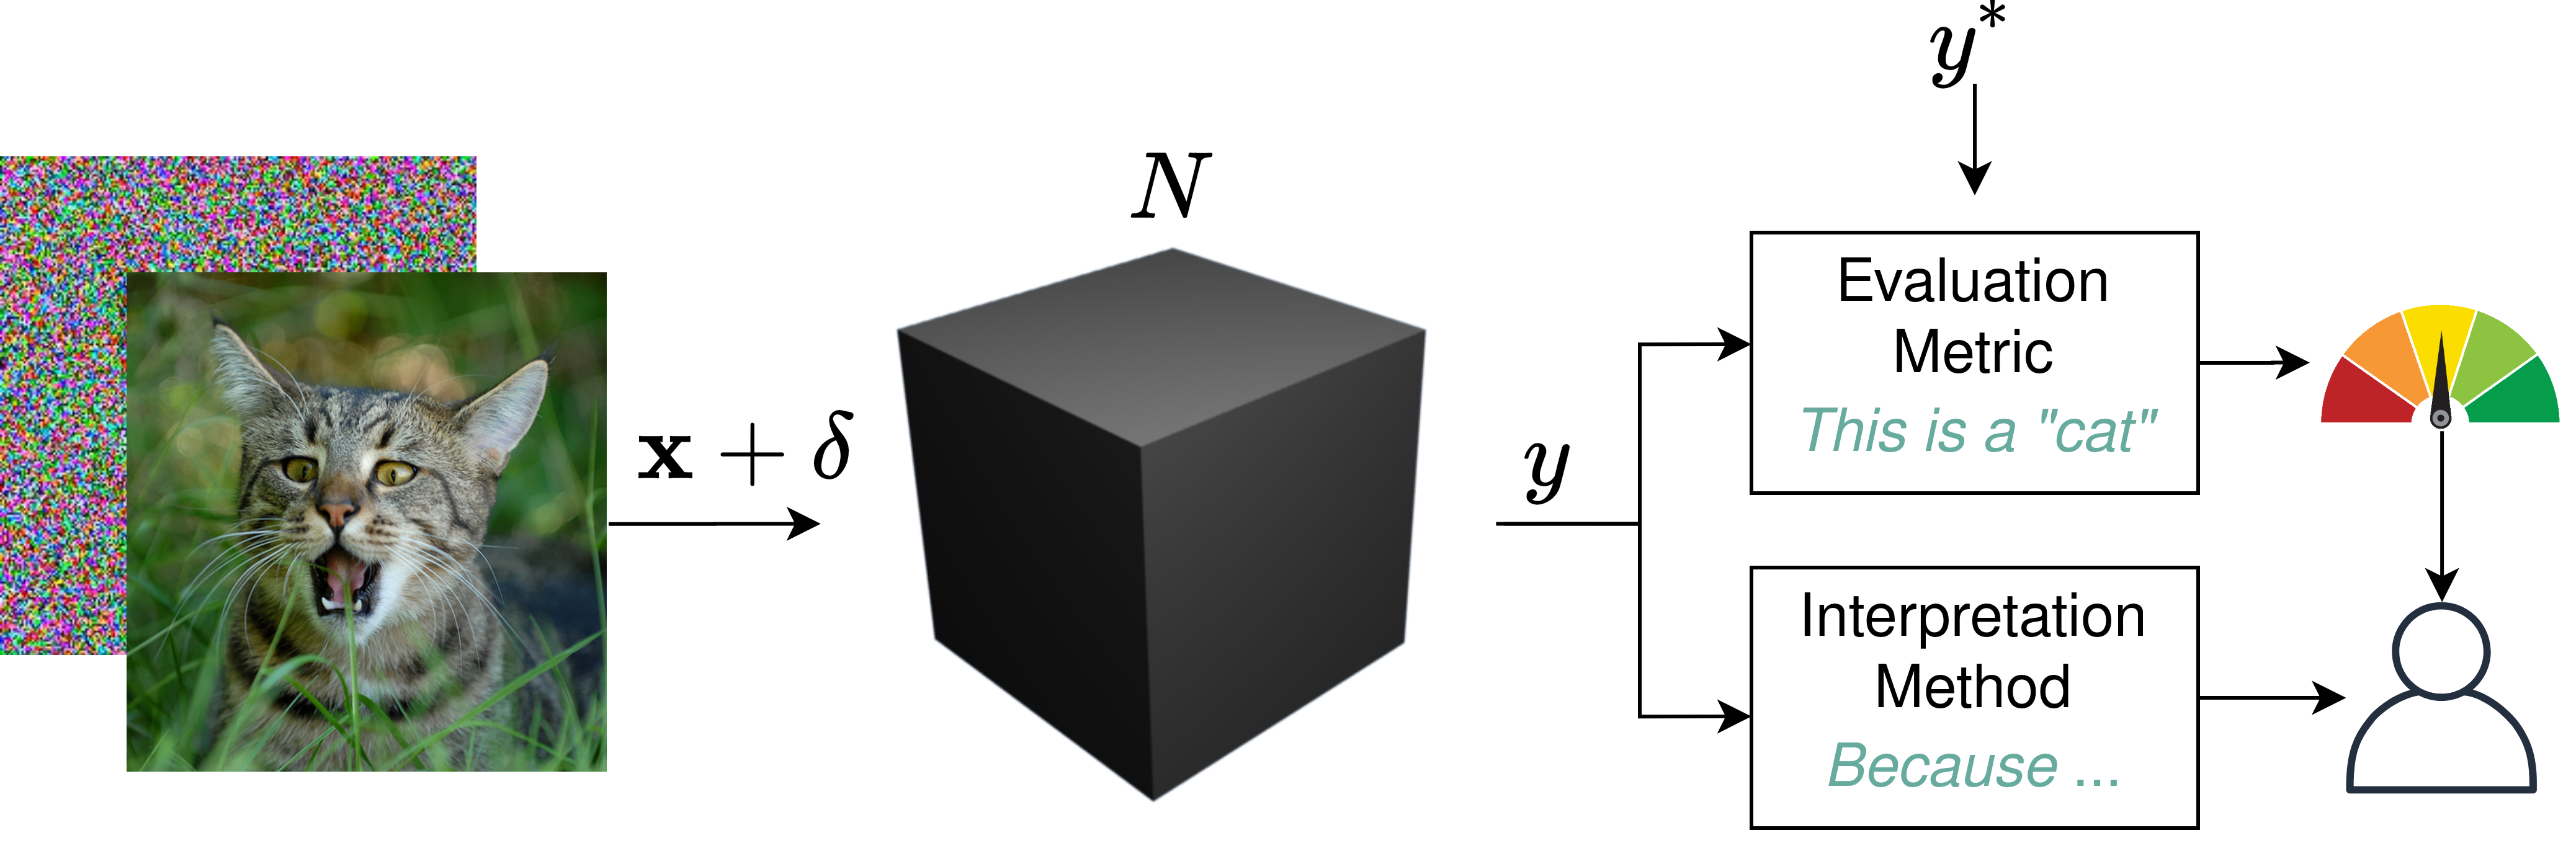
\includegraphics[width=\linewidth]{figures/input_manipulations.png}
    \caption{Depiction of an adversarial input manipulation. The model is fine-tuned with altered input samples, which are indicated by $\mathbf{x}+\delta$.}
    \label{fig:input_manipulation}
    \vspace{-0.3cm}
\end{figure}

\par\smallskip
\noindent\textbf{Adversarial Model Manipulation.} 
Contrary to input manipulations, model manipulations do not operate on the input space but rather on the model parameter space itself. 
As first introduced by Heo et al. \cite{fooling_nn_interpreters} in 2019, this line of research is comparably new. 
Adversarial model manipulations for fooling the interpreter are obtained by fine-tuning the model on the same data but with an adapted objective function. \cite{fooling_nn_interpreters} propose the adapted loss function for the task of image classification of $$ \mathcal{L} = \mathcal{L}_{CE}(\mathcal{D};\omega) + \lambda \cdot \mathcal{L}(\mathcal{D};\omega; \omega_0) $$ where $\mathcal{L}_{CE}$ is the standard cross-entropy classification loss. 
Adversarial model manipulation
\begin{figure}[ht]
    \centering
    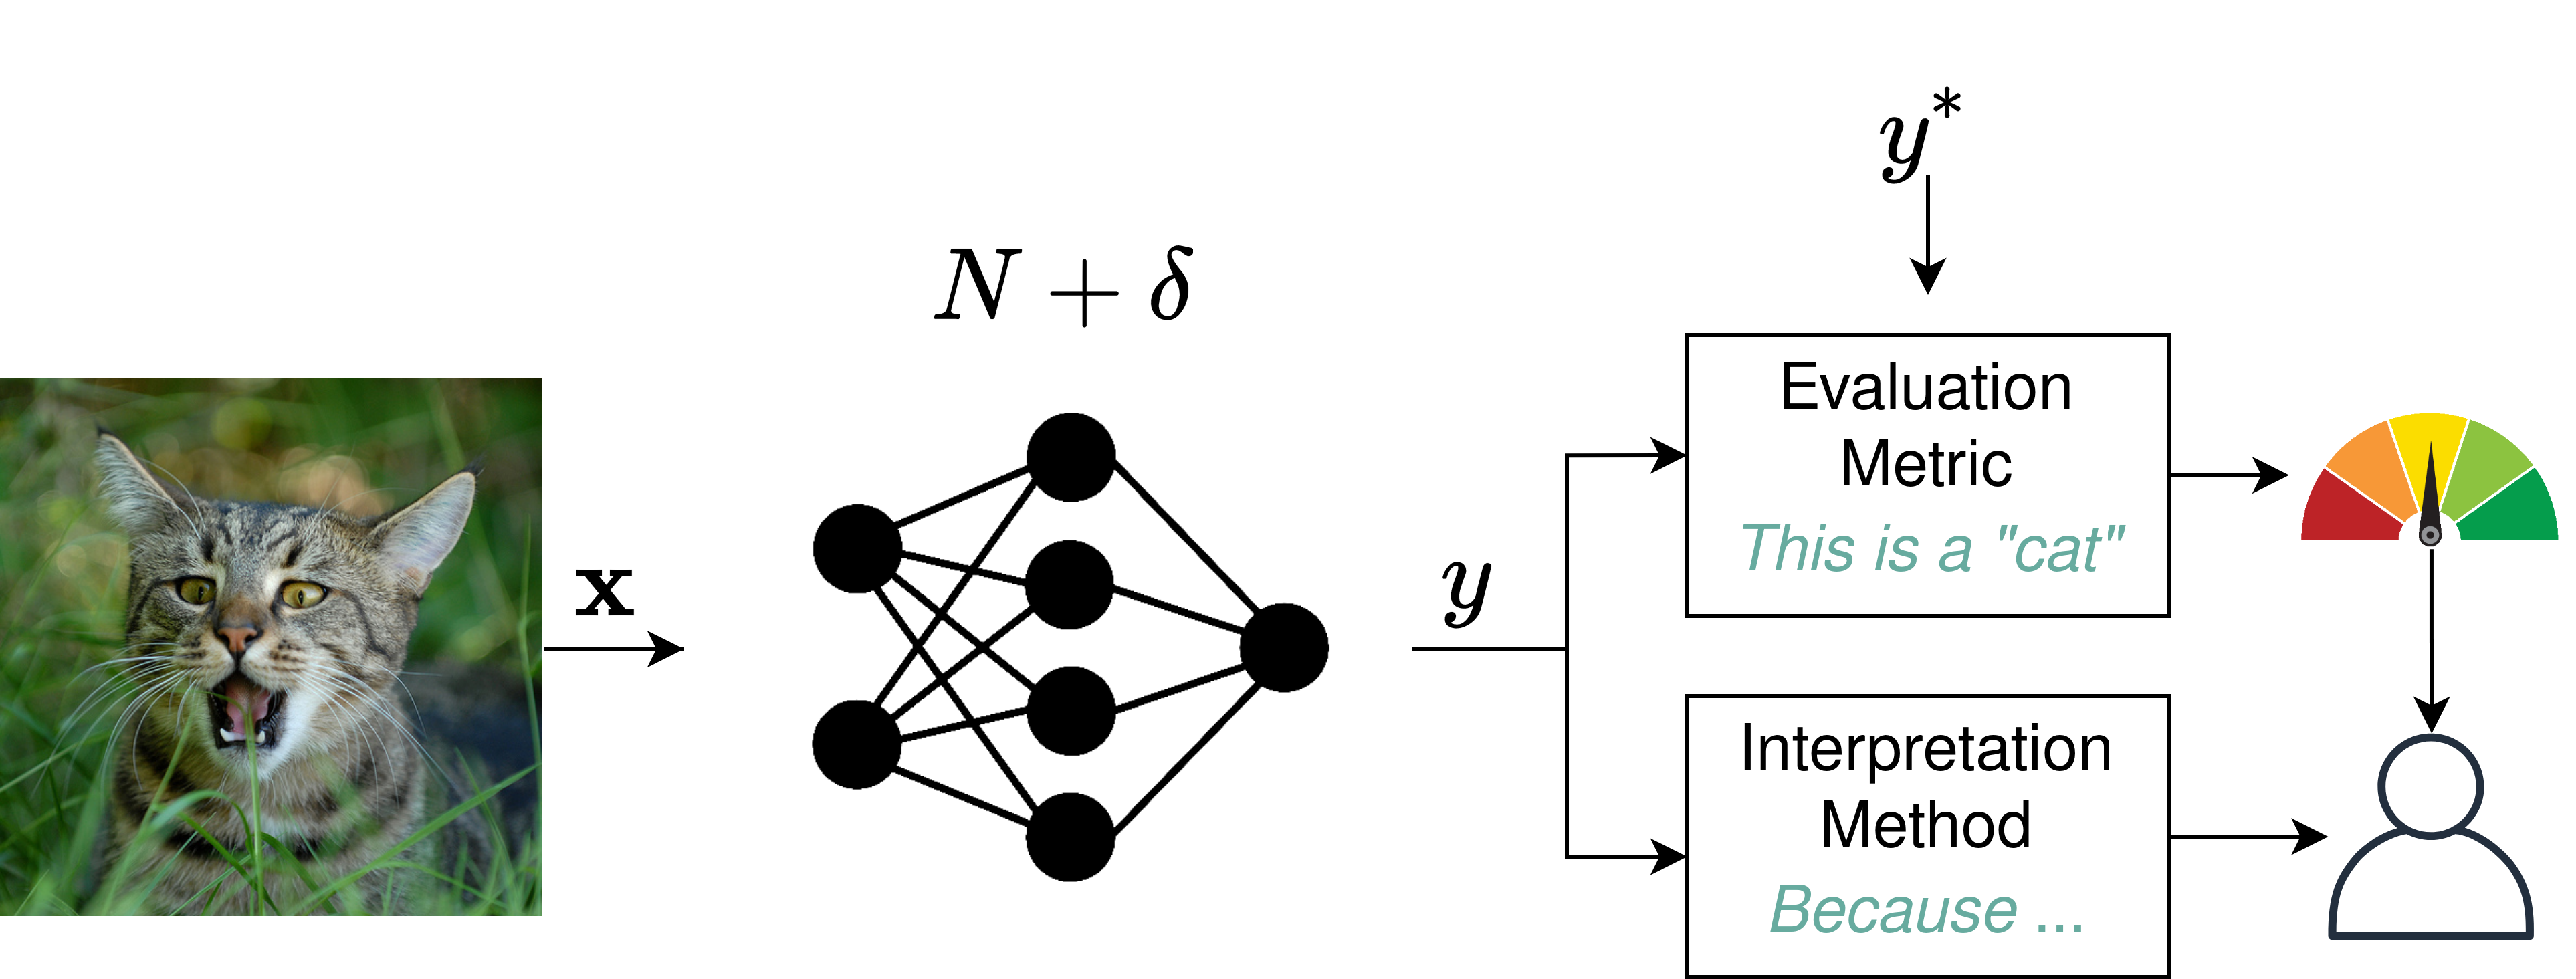
\includegraphics[width=\linewidth]{figures/model_manipulations.png}
    \caption{Depiction of an adversarial model manipulation. The model is fine-tuned with the same distribution of input data and a fooling loss, thus yielding the biased model $N+\delta$.}
    \label{fig:input_manipulation}
    \vspace{-0.3cm}
\end{figure}

%%%%%%%%%%
\subsubsection{Manipulation Targets}
\label{subsubsec:manipulation_targets}

\par\smallskip
\noindent
In addition to the categorization of manipulation methods based on the manipulation level, the methods can further be categorized based on the target of their perturbation. The first possibility is \textit{untargeted} perturbation, the second is \textit{targeted} perturbation. Both these styles can be applied on either model and input level. 

\mypar{Untargeted Manipulations.} 
The majority of manipulations is untargeted, meaning that the applied perturbations are mostly random and not designed to change the prediction for a specific portion of an input sample. 

\mypar{Targeted Manipulations.} 
On the contrary, targeted manipulations aim at specifically changing the explanation of certain features of an input instance \cite{fooling_nn_interpreters}, and sometimes even changing the interpretation of specific classes \cite{simonyan2013deep}. Such a specific feature might be an object in the input image in the context of image classification. \cite{fooling_nn_interpreters} for instance introduce a fooling scheme in which the interpretations of the target classes elephant and school bus are swapped. 
Manipulations on the level of the model are mostly targeted, as the explanation methods are being fooled by adapting the model parameters. 

% Model manipulations pose a much higher threat for deploying the models: If a model itself is changed to explicitly, systemactically fool an explanation method, the bias of the model is internal and much harder to reveal than just a different sort of input into the model. 

%%%%%%%%%%%%%%%%%%%%%%%%% 
\subsection{Evaluation Criteria}
\label{subsec:eval_criteria_manipulations}
Besides the necessary properties of a successful interpretation manipulation method, other evaluation criteria are important to access the success of a fooling method as well as to enable the comparison between different fooling methods. These criteria are informally defined in the following.

\mypar{Effectiveness.} The manipulation scheme is inexpensive to conduct. Input manipulations are by definition inexpensive, as the perturbation can be applied to single input samples. Model manipulations are more expensive as they require tho model parameters to be adapted. However, an adversarial model can be obtained by fine-tuning the model with an adapted objective function. This fine-tuning also has the advantage that the model is adapted to include a systematic bias and can thus be applied to fool explanation methods without further adapting the model or input samples after the fine-tuning step. Furthermore, this systematic bias is hidden in the model, and is hard to uncover. Input manipulations can only fool the model when the inputs are always manipulated. 

\mypar{Transferability.} The manipulation does not only fool one type of interpretation method, but it's effect transfers to other interpretation techniques. 
% This property is naturally given for the class of model manipulations

\mypar{Stability.} The manipulation method influences the interpretation method consistently in a similar way in independent runs. 

\mypar{Generalisation.} Generalization of an attack refers to the transfer of fooling to other test samples. This is noteworthy since a manipulation method might only perturb the decision boundary locally around the training points, i.e. only influencing training instances and their neighbors. However, it is desired that the explanations of unseen samples are affected as well. Furthermore, not only unseen samples interpretations, but also samples that are far away in the feature space should be affected. 
Otherwise, the perturbation is only local around the training points, thus the perturbation does not generalize. 

\par\smallskip
As outlined in section \autoref{sec:manipulation_methods}, there exists a plethora of interpretation methods differing in the assumption about the model character and also with respect to how interpretations are obtained. Thus, reliable evaluation methods are required allowing for a choice of an appropriate and robust interpretation method. Ultimately, the accordance to these evaluations should naturally allow for choosing an appropriate and robust interpretation method.  
Evaluations of the quality of an explanation method are separated into qualitative and quantitative evaluations. 

\mypar{Qualitative Evaluation.} 
Inspection and random sampling are commonly used techniques to obtain an intuition about the effect of manipulations. 
As interpretations are attributed to input features, the resulting relevance values $l$ can be easily mapped to the input vector $\mathbf{x}$. Visual inspection of these evaluations for specific samples is informative, but does not allow for general statistics and validation of manipulation effects. Thus, quantitative evaluations are required. 
\cite{adebayo2018sanity} consider two kinds of visualizing saliency maps: 
\begin{itemize}
    \item \textbf{Absolute Value (ABS).} Saliency maps visualized this way show only the absolute values of the normalized maps.
    \item \textbf{Diverging. } The diverging visualization indicates positive and negative importance in different colors. 
\end{itemize}

\mypar{Quantitative Evaluation.} 
As the goal of interpreter manipulations is to fool an interpreter, thus altering the output of in interpreter, it is straightforward to compare interpretations and data samples before and after perturbation \cite{ghorbani2019interpretation}.

As interpreter manipulations shall alter the output of an interpretation methods while keeping the prediction of a model unchanged, the following metrics 

\begin{itemize}
    \item \textbf{Fooling Success Rate (FSR).} \cite{fooling_nn_interpreters} introduce the concept of the Fooling Success Rate (FSR). The FSR captures the relationship between the model's predictive accuracy and the correctness of the interpretation averaged over multiple test samples. The 'correctness' of the interpretation is the difference between the original interpretation methods output and the output of the same interpretation method when applied to either an adversarial input sample or adversarial model. 
    The FSR counts samples for the model's prediction did not change but for which the interpretation method's output changed as a successfully fooled example. Thus, the higher the FSR, the the more often the fooling is successful in fooling the interpretation method. 
    \item \textbf{Area Over Prediction Curve (AOPC). } AOPC \cite{samek2016evaluating} is a principled way of quantitatively evaluating that the interpretations found by interpretation methods are valid, i.e. based on the features that the model truly uses for making the prediction. \cite{fooling_nn_interpreters} use this measure to ensure that their adversarial model training does not fool the model (i.e. the predictive accuracy of the model is unchanged), but does fool the interpretation method.
\end{itemize}

As the goal of interpreter manipulations is to fool an interpreter, thus altering the output of in interpreter, it is straightforward to compare interpretations and data samples before and after perturbation \cite{ghorbani2019interpretation}.
There are metrics that are applied to identify changes in salient features for any task:
\begin{itemize}
    \item \textbf{Spearman's rank order correlation.} As interpretation methods rank the features based on their importance, the rank correlation \cite{spearman1961proof} is a natural measure for comparing interpretations. 
    \item \textbf{Intersection of the top-$k$ features.} For some tasks, only the top-$k$ features are relevant, such that a comparison between these top-$k$ features is insightful. 
\end{itemize}

Contrary, the following metrics are used only in computer vision tasks. They have been used in literature to quantify similarities between natural images and remove duplicates. Therefore, they are used in XAI research to compare the changes between saliency maps before and after manipulation for computer vision tasks.
\begin{itemize}
    \item \textbf{Structural Similarity Index (SSIM).} SSIM values are relative similarity measure in the range $\left[0, 1\right]$, where larger values indicate higher similarity.
    \item \textbf{Pearson Correlation Coefficient (PCC).} PCC is also a relative similarity measure returning values in the range $\left[0, 1\right]$. Larger values indicate higher similarity.
    \item \textbf{Pearson Correlation of the Histogram of Gradients\newline (HOG). } Used by \cite{adebayo2018sanity} to indicate the intensity of change between two images. 
    \item \textbf{Mean Squared Error (MSE).} As an absolute error measure, values close to zero indicate high similarity. 
\end{itemize}

\noindent Note that these are only examples without demand for completeness. For further information see \cite{adebayo2018sanity}.
Normalizing these measures to yield values in $\left[0, 1\right]$ with a sum of one is good practice. 
Note that defining similarities that are similar to human vision is still an active area of research. 